\documentclass[12pt]{article}

\usepackage[left=3.5cm, right=3.5cm]{geometry}
\usepackage{minted}
\usepackage{listings}
\usepackage{hyphenat}
\usepackage{float}
\usepackage[T1]{fontenc}
\usepackage{hyperref,adjustbox}
\usepackage{graphicx}
\usepackage{pdfpages}
\usepackage[brazilian]{babel}
\usepackage{adjustbox}
\usepackage{multirow}
\usepackage{amssymb}
\usepackage{tabulary}
\usepackage{pifont}% http://ctan.org/pkg/pifont
\newcommand{\cmark}{\ding{51}}%
\newcommand{\xmark}{\ding{55}}%
\usepackage{tikz}
\usepackage{natbib}
\usepackage[T1]{fontenc}
\usepackage{bm}
\usepackage{enumitem}
\usepackage{algorithm}
%\usepackage{arevmath}     % For math symbols
\usepackage[noend]{algpseudocode}
\usepackage{mathtools}

\usepackage{titlesec}
\DeclarePairedDelimiter\ceil{\lceil}{\rceil}
\DeclarePairedDelimiter\floor{\lfloor}{\rfloor}

\titleformat{\section}
{\normalfont\Large\bfseries}{\thesection}{1em}{}[{\titlerule[0.8pt]}]


\title{Trabalho Prático 2 -- Simulação de um Ecossistema \\
	\large Computação Paralela}

\author{Heitor L. Werneck}
\begin{document}
\maketitle

\section{Introdução}

Com o avanço das tecnologias de computação pesquisadores cada vez mais utilizam modelos de simuladores para diversas finalidades, na qual podemos destacar a análise e visualização das conexões complexas que emergem das simulações.

Os sistemas biológicos manifestam muitos exemplos importantes de propriedades emergentes na complexa interação de componentes. O estudo tradicional de sistemas biológicos requer métodos redutivos nos quais as quantidades de dados são reunidas por categoria, deste modo os computadores são essenciais para a análise e modelagem desses dados.

Então, neste trabalho o problema a ser resolvido consiste na simulação de um ecossistema simples,
habitado por duas espécies de animais, raposas e coelhos, cuja existência ao longo de gerações é mutuamente dependente.

Nesse trabalho será apresentado a proposta serial e a paralela para ambientes de memória compartilhada para solucionar o problema, que foram feitas usando C e a interface de programação paralela de memória compartilhada multiplataforma OpenMP. A simulação é feita seguindo as especificações definidas no documento de descrição do trabalho prático.

A próxima seção apresentará as estruturas de dados e toda implementação feita em C. Após isso será discutido a solução paralela proposta. Já na quarta seção será apresentado os resultados obtidos, junto com discussões dos resultados, impacto da variação dos parâmetros e da carga, uso de recursos computacionais, perfil de desempenho sequencial, discussão da identificação das oportunidades de paralelização e avaliação dos ganhos da paralelização. Por fim é feito uma conclusão do trabalho com discussões sobre os resultados e trabalhos futuros que podem ser explorados.

\section{Implementação}

Nesa seção será introduzido os módulos com suas respectivas estruturas de dados e funções.

\subsection{Módulo de erros (errors)}

Esse é o módulo mais simples do código criado, ele somente contém a definição de dois erros utilizados.

\subsubsection{Estrutura de dados}

\begin{minted}{c}
typedef enum
{
    E_SUCCESS, // Sucesso
    E_OUT_OF_BOUNDS // Acesso a algo fora do espaço de memória reservado
}error_t;
\end{minted}

\subsection{Módulo de utilitários (utils)}

Esse é o módulo que contém as funções utilitárias dos programas, trata entrada e saída de dados assim como algumas transformações de dados.


\begin{minted}[tabsize=2,breaklines]{c}
  char *rf_ecosystem_object_type_to_string(rf_ecosystem_object_type_t object_type);
\end{minted}

Transforma um tipo de objeto do ecosistema em uma string. object\_type é um tipo de objeto a ser ''transformado'' em uma string. O retorno é uma string que representa um tipo de objeto.

\begin{minted}[tabsize=2,breaklines]{c}
rf_ecosystem_object_type_t string_to_rf_ecosystem_object_type(char *string_buffer);
\end{minted}

Transforma um tipo de objeto do ecosistema em uma string. string\_buffer é uma string que representa um tipo de objeto. string\_buffer é uma string que representa um tipo de objeto. O retorno é um tipo de objeto rf\_ecosystem\_object\_type\_t correspondente a string\_buffer.

\begin{minted}[tabsize=2,breaklines]{c}
      rf_ecosystem_object_type_t string_to_rf_ecosystem_object_type(char *string_buffer);
      \end{minted}

Transforma um tipo de objeto do ecosistema em uma string. string\_buffer é uma string que representa um tipo de objeto. string\_buffer é uma string que representa um tipo de objeto. O retorno é um tipo de objeto rf\_ecosystem\_object\_type\_t correspondente a string\_buffer.


\begin{minted}[tabsize=2,breaklines]{c}
void print_ecosystem_full_report(rf_ecosystem_t *es);
      \end{minted}

Imprime o ecosistema na saída padrão no formato esperado definido na especificação. es é o ecosistema para ser imprimido.

\begin{minted}[tabsize=2,breaklines]{c}
rf_ecosystem_t *initial_setup();
      \end{minted}

Faz a configuração inicial dos programas, no qual é feito uma leitura da entrada padrão e criado o ecosistema inicial de acordo com a entrada. A função retorna o ecossistema carregado da entrada padrão.

\subsection{Módulo de simulação de coelhos e raposas (rabbits\_fox)}

Este pacote provê todo o código, com funções e estruturas de dados, para realizar as simulações de maneira paralela (usando OpenMP) e serial.

\subsubsection{Estrutura de dados e Variáveis Globais}

Agora será apresentado as estruturas de dados desse módulo, as estruturas compreendem diversos aspectos do ecossistema, como: objetos, ecosistema, direções e outros.


\begin{minted}[tabsize=2,breaklines]{c}
typedef struct {
  int procreation_age, food_generations;
  rf_ecosystem_object_type_t type;
  int previous_line, previous_column;
} rf_ecosystem_object_t;
      \end{minted}

Este é a estrutura que representa um objeto do ecossistema, que pode ser nada, um coelho, uma raposa, ou uma rocha. Ele contém os atributos em relação à fome, reprodução e coordenadas do objeto.

\begin{minted}[tabsize=2,breaklines]{c}
typedef enum {
  RF_EMPTY = ' ',// tipo vazio
  RF_RABBIT = 'C',// tipo coelho
  RF_FOX = 'R',// tipo raposa
  RF_ROCK = '*'// tipo rocha
} rf_ecosystem_object_type_t;
      \end{minted}

Esse enum define os tipos de objeto do ecossistema, que ficam no ambiente.

\begin{minted}[tabsize=2,breaklines]{c}
typedef struct {
  int procreation_age, food_generations;
  rf_ecosystem_object_type_t type;
  int previous_line, previous_column;
} rf_ecosystem_object_t;
      \end{minted}

Já essa estrutura de dados define objeto do ecossistema, que fica no ambiente, que pode ser nada, um coelho, uma raposa, ou uma rocha. Ele contém os atributos em relação à fome, reprodução e coordenadas do objeto.

\begin{minted}[tabsize=2,breaklines]{c}
typedef struct  {
  int GEN_PROC_COELHOS, GEN_PROC_RAPOSAS, GEN_COMIDA_RAPOSAS, N_GEN, L, C, N;
  int current_generation;// geração corrente
  rf_ecosystem_object_t **environment;// ambiente com os objetos
}rf_ecosystem_t;
      \end{minted}


Já essa estrutura define o ecossistema que contém os parâmetros para simulação incluindo o próprio ambiente com as raposas, coelhos e rochas.

\begin{minted}[tabsize=2,breaklines]{c}
omp_lock_t **LOCK_MATRIX;
int COUNTER;
      \end{minted}

O LOCK\_MATRIX é uma matriz de lock que indica uma região do ambiente que está sendo acessado ou escrito, é utilizado na implementação paralela e deixa o código mais legível, e sem modificações que são somente necessárias para a solução paralela, sendo uma variável global.
O COUNTER é um contador utilizado em algumas funções, está sendo usado como uma variável global, pois deixa o código mais legível com a implementação paralela e sem modificações só necessárias para a solução paralela.


\begin{minted}[tabsize=2,breaklines]{c}
#define DIRECTIONS_NUMBER 4
#define next_cell(g, x, y, p) (((g) + (x) + (y)) % (p))
typedef enum { NORTH, EAST, SOUTH, WEST } directions_t;
const directions_t directions_order[] = {NORTH, EAST, SOUTH, WEST};
      \end{minted}

O DIRECTIONS\_NUMBER é o número de direções, isto é, norte, leste, sul, oeste.

O directions\_t define o tipo de direções que também são as direções que as raposas e coelhos podem se mover, isto é: norte; leste; sul; e oeste.

O directions\_order define a ordem das direções no vetor de enumeração de direções disponíveis.

\subsubsection{Funções}

Agora será descrito as funções do pacote de simulação. O pacote consiste em alguns utilitários, funções para atualização dos coelhos e raposas entre outras funções.

\begin{minted}[tabsize=2,breaklines]{c}
void _direction_adjacent_cell(directions_t direction, int *line, int *column);
      \end{minted}

Essa função obtém a linha e a coluna dado uma linha, coluna e uma direção. direction é a direção que irá determinar a próxima linha e coluna. line é a linha base para ser modificada dada a direção escolhida. column é a coluna base para ser modificada dada a direção escolhida.

\begin{minted}[tabsize=2,breaklines]{c}
rf_ecosystem_t *rf_new_ecosystem(int GEN_PROC_COELHOS, int GEN_PROC_RAPOSAS,
                                 int GEN_COMIDA_RAPOSAS, int N_GEN, int L,
                                 int C, int N);
      \end{minted}

Cria um ecossistema dado os parâmetros.
GEN\_PROC\_COELHOS é o número de gerações até que um coelho possa procriar.
GEN\_PROC\_RAPOSAS é o número de gerações até que uma raposa possa procriar.
GEN\_COMIDA\_RAPOSAS é o número de gerações para uma raposa ficar com fome.
N\_GEN é o número de gerações para a simulação
L é o número de linhas da matriz representando o ecossistema
C é o número de colunas da matriz representando o ecossistema
N é o número de objetos no ecossistema inicial
A função retorna o ecossistema criado com base nos parâmetros passados.


\begin{minted}[tabsize=2,breaklines]{c}
rf_ecosystem_t *rf_clone_ecosystem(rf_ecosystem_t *es);
      \end{minted}

A função faz um clone de um ecossistema preexistente.
es é o ambiente a ser duplicado.
A função retorna o ambiente duplicado.

\begin{minted}[tabsize=2,breaklines]{c}
void rf_clear_environment(rf_ecosystem_t *es);
      \end{minted}

Esta é a função que limpa os objetos vivos do ambiente.
es é o ecossistema a ter seu ambiente limpo.


\begin{minted}[tabsize=2,breaklines]{c}
void rf_insert_object_ecosystem(rf_ecosystem_t *es, rf_ecosystem_object_t obj,
                                int x, int y);
      \end{minted}

Esta é a função que insere um novo objeto no ecossistema.
es é o ecossistema a ter um objeto inserido.
obj é o objeto a ser inserido.
x é a linha onde o objeto será inserido.
y é a coluna onde o objeto será inserido.


\begin{minted}[tabsize=2,breaklines]{c}
void rf_free_ecosystem(rf_ecosystem_t *es);
      \end{minted}

Libera o espaço de memória reservado para o ecossistema.
es é o ecossistema a ter a memória liberada.

\begin{minted}[tabsize=2,breaklines]{c}
void rf_print_ecosystem_environment(rf_ecosystem_t *es);
      \end{minted}

Esta é a função que imprime o ambiente (matriz) do ecossistema com os objetos.
es é o ambiente a ter o ambiente imprimido.

\begin{minted}[tabsize=2,breaklines]{c}
rf_ecosystem_object_t *rf_get_ecosystem_object(rf_ecosystem_t *es, int x, int y,
                                               error_t *status);
      \end{minted}

Essa função obtém um objeto do ambiente.
es é o ambiente a ter o objeto obtido.
x é a linha do objeto a ser obtido.
y é a coluna do objeto a ser obtido.
status é o status da obtenção do objeto, no caso pode haver um erro se for além dos limites do mundo.
A função retorna o objeto.


\begin{minted}[tabsize=2,breaklines]{c}
void rf_enumerate_directions(rf_ecosystem_t *es, int *directions_available,
                             int *directions_counter, int line, int column,
                             rf_ecosystem_object_type_t obj_to_search_type);
      \end{minted}

Esta função enumera as células que não tem objetos de um certo tipo dado nas 4 direções.
es é o ambiente.
directions\_available são as direções disponíveis que serão preenchidas na função.
directions\_counter é a enumeração das direções disponíveis que serão preenchidas na função.
line é a linha a ser avaliada as células adjacentes.
column é a coluna a ser avaliada as células adjacentes.
obj\_to\_search\_type é o tipo de objeto a ser procurado.



\begin{minted}[tabsize=2,breaklines]{c}
void rf_update_ecosystem_rabbits(rf_ecosystem_t *es,
                                 rf_ecosystem_t *buffer_es);
      \end{minted}

Essa função atualiza os coelhos do ecossistema conforme as regras definidas na especificação.
es é o ecossistema base.
buffer\_es é o ecossistema que serve como um buffer para posterior atualização do ecossistema base.



\begin{minted}[tabsize=2,breaklines]{c}
void rf_update_ecosystem_foxes(rf_ecosystem_t *es, rf_ecosystem_t *buffer_es);
      \end{minted}


Essa função atualiza as raposas do ecossistema conforme as regras definidas na especificação.
es é o ecossistema base.
buffer\_es é o ecossistema que serve como um buffer para posterior atualização do ecossistema base.

\begin{minted}[tabsize=2,breaklines]{c}
void rf_update_ecosystem_rabbits_from_buffer(rf_ecosystem_t *es,
                                             rf_ecosystem_t *buffer_es);
      \end{minted}

Essa função atualiza os coelhos do ecossistema para o ecossistema base.
es é o ecossistema base.
buffer\_es é o ecossistema que serve como um buffer que terá seus dados transferidos para o ecossistema base.



\begin{minted}[tabsize=2,breaklines]{c}
void rf_update_ecosystem_foxes_from_buffer(rf_ecosystem_t *es,
                                           rf_ecosystem_t *buffer_es);
      \end{minted}

Essa função atualiza as raposas do ecossistema para o ecossistema base.
es é o ecossistema base.
buffer\_es é o ecossistema que serve como um buffer que terá seus dados transferidos para o ecossistema base.


\begin{minted}[tabsize=2,breaklines]{c}
void rf_update_ecosystem_generation(rf_ecosystem_t *es,
                                    rf_ecosystem_t *buffer_es);
      \end{minted}

Essa função atualiza o ecossistema de maneira geral em uma geração.
es é o ecossistema base.
buffer\_es é o ecossistema que serve como um buffer.


\begin{minted}[tabsize=2,breaklines]{c}
rf_ecosystem_t *rf_update_ecosystem_generations(rf_ecosystem_t *es);
      \end{minted}


Essa função atualiza o ecossistema de maneira geral com base nas gerações do ecossistema base de entrada.
es é o ecossistema base.
buffer\_es é o ecossistema que serve como um buffer.


\subsection{main}

Esse é um código principal, chamado main.c, que contém a implementação principal do programa. Através de diretivas de compilação foi possível compilar o programa serial e o paralelo usando somente um código principal. O mesmo utiliza o módulo de simulação e de utilitários descritos anteriormente.

\section{Solução Paralela}

Com a execução da abordagem serial foi possível obter algumas informações sobre oportunidades de paralelização, mais informações sobre os resultados serão detalhados em uma futura seção, por enquanto será focado na solução proposta.

Com execução e análise usando o perfil sequencial da execução junto com o conhecimento sobre a estrutura do código foi visto uma oportunidade de paralelização, que consiste na paralelização por linhas (vertical) da matriz do ambiente para os Workers. A paralelização foi feita de modo bem flexível, deste modo é possível usar todos escalonadores do OpenMP.

Essa paralelização foi feita usando uma matriz de lock, no qual cada linha e coluna, quando acessada para escrita ou leitura, será ativada (set) na matriz de lock para que nenhum outro Worker faça algum acesso, deste modo evitando condições de corrida.

Essa solução pode ser otimizada para casos específicos de escalonamento, porém para explorar todos escalonadores do OpenMP e gerar uma análise mais interessante foi feito essa abordagem genérica para qualquer escalonador e sem nenhuma pressuposição sobre a carga de trabalho, onde os Workers sempre fazem o lock quando acessam, que em casos específicos de escalonamento, como no escalonamento estático de blocos contíguos pode ser otimizado e o lock pode ser feito somente nas ''bordas''.

Essa paralelização foi pensada pela sua natureza paralela, que no entando tem seus problemas devido à dependência a células adjacentes de outros Workers.

No caso, com a utilização do OpenMP para paralelização foi modificado as seguintes funções:

\begin{minted}[tabsize=2,breaklines]{c}
void rf_clear_environment(rf_ecosystem_t *es);
void rf_update_ecosystem_rabbits(rf_ecosystem_t *es,
                                 rf_ecosystem_t *buffer_es);
void rf_update_ecosystem_foxes(rf_ecosystem_t *es, rf_ecosystem_t *buffer_es);
void rf_update_ecosystem_rabbits_from_buffer(rf_ecosystem_t *es,
                                             rf_ecosystem_t *buffer_es);
void rf_update_ecosystem_foxes_from_buffer(rf_ecosystem_t *es,
                                           rf_ecosystem_t *buffer_es);
void rf_update_ecosystem_generation(rf_ecosystem_t *es,
                                    rf_ecosystem_t *buffer_es);
rf_ecosystem_t *rf_update_ecosystem_generations(rf_ecosystem_t *es);
      \end{minted}


Então, resumindo as modificações incluém: inclusão da diretiva de distribuição do for do OpenMP; somas em variáveis são resolvidas usando a cláusula de redução; matriz de lock; lock's feitos de maneira adequada nas funções
rf\_update\_ecosystem\_foxes e
rf\_update\_ecosystem\_rabbits; barreiras para sincronização; e mais algumas pequenas modificações que podem ser vistas na implementação.





\section{Resultados e Análises}
\subsection{Execução Simples}

Aqui será mostrado um simples caso de entrada e saída do programa que demonstra como o mesmo funciona e como se comporta. Veja a seguir a execução do programa:

\begin{verbatim}
$ ./serial-rabbits-and-foxes < data/in/example.txt > data/out/example.txt 
$ pr -m -t ./data/in/example.txt ./data/out/example.txt | head            
2 4 3 6 5 5 9                       2 4 3 0 5 5 5
ROCHA 0 0                           ROCHA 0 0
COELHO 0 2                          ROCHA 2 4
RAPOSA 0 4                          COELHO 3 0
RAPOSA 1 0                          RAPOSA 4 0
RAPOSA 1 4                          RAPOSA 4 3
ROCHA 2 4                           
COELHO 3 0                          
COELHO 4 0                          
RAPOSA 4 4                      
\end{verbatim}


Esse exemplo executado é o apresentado na especificação e é possível ver que o simulador conseguiu o mesmo resultado. Para ver o tempo de execução é necessário utilizar o commando ''make release\_debug\_time'' para compilar o programa com essa funcionalidade.

\subsection{Memória}

Para verificação de qualquer vazamento de memória foi utilizado o \textit{Valgrind}. Como pode ser visto abaixo, em uma execução normal não existe nenhum problema em relação à vazamento de memória com o programa.

	{
		\scriptsize
		\begin{verbatim}
==54761== Memcheck, a memory error detector
==54761== Copyright (C) 2002-2017, and GNU GPL'd, by Julian Seward et al.
==54761== Using Valgrind-3.17.0 and LibVEX; rerun with -h for copyright info
==54761== Command: ./serial-rabbits-and-foxes
==54761== 
==54761== 
==54761== HEAP SUMMARY:
==54761==     in use at exit: 0 bytes in 0 blocks
==54761==   total heap usage: 16 allocs, 16 frees, 9,352 bytes allocated
==54761== 
==54761== All heap blocks were freed -- no leaks are possible
==54761== 
==54761== For lists of detected and suppressed errors, rerun with: -s
==54761== ERROR SUMMARY: 0 errors from 0 contexts (suppressed: 0 from 0)
\end{verbatim}
	}

Além disso, o programa paralelo não foi possível ser testado, já que o OpenMP possui vazamentos de memória, o que dificulta a utilização do \textit{Valgrind}. Apesar disso o código foi revisado e não foi encontrado nenhum possível vazamento. Além disso os vazamentos observados não são danosos ao programa.

\subsection{Perfil de Desempenho Sequencial}

Para avaliação do desempenho sequencial foi avaliado uma entrada com os parâmetros descritos na tabela a seguir:


\begin{table}[H]
	\begin{center}
		\begin{tabular}{|l|c|}
			\hline
			Parâmetro                           & Valor \\
			\hline
			GEN\_PROC\_COELHOS                  & 2     \\
			GEN\_PROC\_RAPOSAS                  & 4     \\
			GEN\_COMIDA\_RAPOSAS                & 3     \\
			L                                   & 10000 \\
			C                                   & 10000 \\
			N                                   & 10000 \\
			N\_GEN                              & 10    \\\hline
			Probabilidade de geração de coelho  & 40\%  \\
			Probabilidade de geração de raposas & 40\%  \\
			Probabilidade de geração de rochas  & 40\%  \\
			\hline
		\end{tabular}
	\end{center}
	\caption{Parâmetros da base de dados para o perfil sequêncial.}
	\label{tab:parametros_base_de_dados_perfil_sequencial}
\end{table}

Muitos dos parâmetros já foram especificados na especificação do trabalho e também já foi mencionado aqui neste trabalho. As probabilidades de geração são variáveis do gerador aleatório de bases de dados utilizado para fazer experimentos em bases de dados maiores utilizado ao longo de todo esse trabalho.


Abaixo está o resultada do perfil de desempenho sequencial do programa. É possível observar que as funções que fazem a atualização do buffer são as que mais gastam tempo, nas mesmas o for existente não gera nenhum conflito entre os Workers, sendo um grande potencial de paralelização. As funções de atualização do ecossistema com base nas regras da especificação também gastam bastante tempo e podem ser paralelizadas, porém, terá um certo malefício devido aos tratamentos de condições de corrida. Além disso, a função de limpar o ambiente pode ser facilmente paralelizada, sendo ela também uma oportunidade de paralelização embaraçosa como as funções de atualização usando o buffer. É possível observar que o potencial de paralelização representa aproximadamente 90\% do tempo de execução. Não é esperado um speed up linear nesse caso, visto a solução genérica e os locks.

A lei de Amdahl da o seguinte speed up para 12 threads $\frac{1}{1-0.9+\frac{0.9}{12}} = 5.7$, que é um limite superior para o speed up, já que há necessidade de tratamento de condição de corrida vai reduzir um pouco o speed up, porém é importante notar que a fração de tempo aqui (no perfil sequencial) também conta o tempo da impressão que é um erro e além disso a fração do programa que pode ser paralelizada foi feita com base em uma estimativa. Então é esperado que com 12 threads não se tenha um speed up próximo de 5.7, mas sim abaixo disso.

	{
		\scriptsize
		\begin{verbatim}
Each sample counts as 0.01 seconds.
  %   cumulative   self              self     total           
 time   seconds   seconds    calls   s/call   s/call  name    
 29.95      7.39     7.39       10     0.74     0.74  rf_update_ecosystem_foxes_from_buffer
 25.29     13.64     6.24       10     0.62     0.62  rf_update_ecosystem_rabbits_from_buffer
 12.64     16.76     3.12       10     0.31     0.31  rf_update_ecosystem_rabbits
 12.56     19.86     3.10       10     0.31     0.31  rf_update_ecosystem_foxes
 12.52     22.95     3.09       10     0.31     0.31  rf_clear_environment
  5.51     24.31     1.36        1     1.36     1.36  rf_new_ecosystem
  1.46     24.67     0.36        1     0.36     0.36  print_ecosystem_full_report
  0.08     24.69     0.02   138577     0.00     0.00  rf_enumerate_directions
  0.04     24.70     0.01   680890     0.00     0.00  _direction_adjacent_cell
  0.00     24.70     0.00   554308     0.00     0.00  rf_get_ecosystem_object
  0.00     24.70     0.00    30990     0.00     0.00  rf_ecosystem_object_type_to_string
  0.00     24.70     0.00    10000     0.00     0.00  rf_insert_object_ecosystem
  0.00     24.70     0.00    10000     0.00     0.00  string_to_rf_ecosystem_object_type
  0.00     24.70     0.00       10     0.00     1.99  rf_update_ecosystem_generation
  0.00     24.70     0.00        2     0.00     0.00  rf_free_ecosystem
  0.00     24.70     0.00        1     0.00     1.36  initial_setup
  0.00     24.70     0.00        1     0.00     0.00  rf_clone_ecosystem
  0.00     24.70     0.00        1     0.00    22.98  rf_update_ecosystem_generations
\end{verbatim}
	}
\subsubsection{Impacto dos parâmetros}

Agora será analisado o impacto da variação dos parâmetros e da carga no tempo de execução do programa usando o algoritmo serial.

Para ser feito essa análise foi definido um conjunto de parâmetros para ser feito uma execução em grade (i.e., todas combinações dos conjuntos de parâmetros) para entender melhor como cada parâmetro impacta no tempo de computação do algoritmo. O conjunto de parâmetros utilizados para ser feito a busca em grade está descrito na tabela \ref{tab:gradeparam}.

\begin{table}[H]
	\begin{center}
		\begin{tabular}{|c|c|}
			\hline
			Parâmetro                           & Valor              \\
			\hline
			GEN\_PROC\_COELHOS                  & \{2, 4\}           \\
			GEN\_PROC\_RAPOSAS                  & \{4, 6\}           \\
			GEN\_COMIDA\_RAPOSAS                & \{3, 5\}            \\
			L                                   & \{100, 250, 500\}  \\
			C                                   & \{100, 250, 500\}  \\
			N                                   & \{250, 500, 1000\} \\
			N\_GEN                              & \{10, 20\}         \\\hline
			Probabilidade de geração de coelho  & 40\%               \\
			Probabilidade de geração de raposas & 40\%               \\
			Probabilidade de geração de rochas  & 40\%               \\
			\hline
		\end{tabular}
	\end{center}
	\caption{Conjunto de parâmetros e carga para a execução em grade.}
	\label{tab:gradeparam}
\end{table}

A visualização do tempo de execução foi feita usando coordenadas paralelas que é uma maneira comum de visualizar e analisar conjuntos de dados de alta dimensão.



%GEN\_PROC\_COELHOS  
%GEN\_PROC\_RAPOSAS  
%GEN\_COMIDA\_RAPOSAS
%L                   
%C                   
%N                   
%N\_GEN              


Na figura \ref{fig:parallel_coordinates} é possível notar que os parâmetros como 
GEN\_PROC\_COELHOS,
GEN\_PROC\_RAPOSAS e  
GEN\_COMIDA\_RAPOSAS não tem muito impacto no tempo de execução final. Já a carga/parâmetro N parece ter um impacto médio, o que é esperado, já que adiciona um pequena sobrecarga devido ao número de checagens, movimentações, reproduções e etc aumentarem. Os parâmetros L, C e N\_GEN já tem mais impacto, o que é esperado, e quanto maior esses parâmetros mais o tempo computação aumenta significativamente.


\begin{figure}[H]
	\begin{center}
		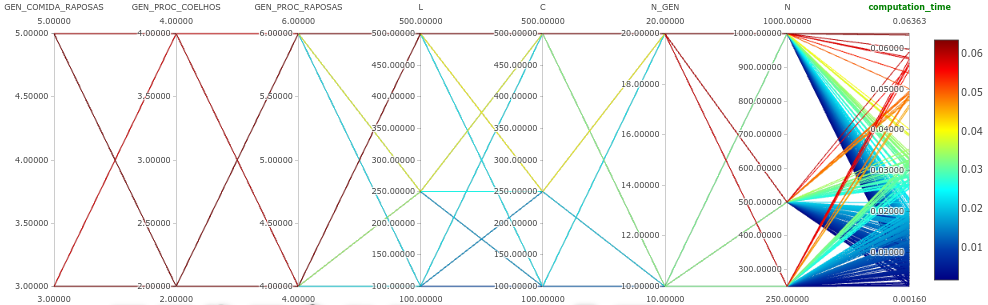
\includegraphics[width=1.0\linewidth]{./parallel_coordinates.png}
	\end{center}
	\caption{Gráfico de coordenadas paralelas do tempo de execução em segundos da versão serial do algoritmo.}
	\label{fig:parallel_coordinates}
\end{figure}


\subsubsection{Recursos computacionais}

Agora serão apresentados os recursos computacionais por parte da aplicação. Esses recursos computacionais foram avaliados usando a base de dados apresentada na tabela \ref{tab:parametros_base_de_dados_perfil_sequencial} usando o comando ''/usr/bin/time -v''. O resultado está apresentado abaixo. É possível notar que uma parte consideravel do tempo de execução é tempo do sistema, porém possivelmente é o tempo de entrada e saída que não está sendo considerado neste trabalho. Agora, sobre o uso máximo de memória residente foi obtido um alto valor de 3921544 kbytes, que é devido principalmente a representação matricial utilizada. Outras abordagens como somente de representação dos objetos presentes no ambiente, sem utilização da matriz poderiam ser utilizados e explorados em trabalhos futuros.


	{
		\scriptsize
		\begin{verbatim}
	Command being timed: "./serial-rabbits-and-foxes"
	User time (seconds): 12.40
	System time (seconds): 2.36
	Percent of CPU this job got: 99%
	Elapsed (wall clock) time (h:mm:ss or m:ss): 0:14.76
	Average shared text size (kbytes): 0
	Average unshared data size (kbytes): 0
	Average stack size (kbytes): 0
	Average total size (kbytes): 0
	Maximum resident set size (kbytes): 3921544
	Average resident set size (kbytes): 0
	Major (requiring I/O) page faults: 0
	Minor (reclaiming a frame) page faults: 980104
	Voluntary context switches: 1
	Involuntary context switches: 16
	Swaps: 0
	File system inputs: 0
	File system outputs: 0
	Socket messages sent: 0
	Socket messages received: 0
	Signals delivered: 0
	Page size (bytes): 4096
	Exit status: 0
\end{verbatim}
	}


\subsection{Ganhos com a Paralelização}

Agora finalmente será abordado os ganhos obtidos com a paralelização e análises de alguns resultados obtidos. Para essa análise será utilizado a base de dados descrita na tabela \ref{tab:parametros_base_de_dados_perfil_sequencial}. Foi executado o programa serial e o paralelo, com diferentes parâmetros do OpenMP. Os resultados são apresentados na tabela \ref{tab:resultados}.

Pela tabela é possível ver que o speed up previsto foi bem abaixo do esperado, mesmo utilizando escalonadores que equilibram dinamicamente a carga. Talvez com uma carga de trabalho maior a abordagem paralela possa aumentar o speed up. O método com menor tempo de execução foi o algoritmo paralelo com o escalonamento guided e chunk size de 400.

Apesar da versão paralela não ter tido um grande melhora no tempo de execução (speed up de 1.4), ainda ela é uma solução melhor que a serial e atingiu o objetivo de pelo menos conseguir diminuir o tempo de execução. Como já discutido anteriormente, uma solução talvez menos flexível, que tenha menos necessidade de tratamento de condição de corrida possa ser mais adequada para esse problema, que pode ser abordado em um futuro trabalho.

%Pela tabela é possível ver que de acordo com o aumento do número de processos na versão paralela "P2", "P3", "P4", e etc há também a diminuição do tempo, em todas as bases parece ter um speed up máximo de 10x com 24 processos. Apesar de ainda não ser próximo do speed up teórico é uma boa melhora. Também é importante notar que como a arquitetura é mestre-escravo quando há 2 processos é quase a mesma coisa que o serial. 


\begin{table}[H]
	\tiny
	\begin{center}
\begin{tabular}{|l|l|l|l|r|}
\hline
 Executável   & Threads   & Política de escalonamento      & Chunk size    & Tempo de execução (segundos)  \\
 \hline\hline
 serial-rabbits-and-foxes   &    &       &     & 13.3376s  \\
 \hline
 parallel-rabbits-and-foxes & 4  & static &     & 11.9403s  \\
 parallel-rabbits-and-foxes & 8  & static &     & 10.147s   \\
 parallel-rabbits-and-foxes & 12 & static &     &  9.49562s \\\hline
 parallel-rabbits-and-foxes & 4  & dynamic&     & 12.3756s  \\
 parallel-rabbits-and-foxes & 8  & dynamic&     & 10.0629s  \\
 parallel-rabbits-and-foxes & 12 & dynamic&     &  9.58124s \\\hline
 parallel-rabbits-and-foxes & 4  & guided &     & 12.8847s  \\
 parallel-rabbits-and-foxes & 8  & guided &     & 10.0421s  \\
 parallel-rabbits-and-foxes & 12 & guided &     &  9.59282s \\
 \hline
 parallel-rabbits-and-foxes & 4  & dynamic& 400 & 13.295s   \\
 parallel-rabbits-and-foxes & 8  & dynamic& 400 & 10.0663s  \\
 parallel-rabbits-and-foxes & 12 & dynamic& 400 &  9.55378s \\\hline
 parallel-rabbits-and-foxes & 4  & guided&400  & 12.4935s  \\
 parallel-rabbits-and-foxes & 8  & guided&400  & 10.2039s  \\
 parallel-rabbits-and-foxes & 12 & guided&400  &  9.46357s \\
\hline
\end{tabular}
\end{center}

	\caption{Algoritmo sequêncial e paralelo com diferentes quantidades de Workers e escalonador.}
	\label{tab:resultados}
\end{table}


\section{Conclusão}

Com este trabalho foi possível ter uma melhor ideia sobre como utilizar o OpenMP na prática e os benéficios do uso. O desenvolvimento do programa paralelo para ambiente de memória compartilhada foi um pouco diferente do trabalho anterior, já que o OpenMP tem uma forma bastante diferente de ser utilizado e trouxe outras prespectivas de como paralelizar o código. Além disso o OpenMP se demonstrou um excelente meio para desenvolvimento de programas paralelos devido a sua facilidade de uso e eficiência.


Os resultados obtidos demonstraram que houve um ganho no uso da computação paralela para resolver o problema, porém esse ganho foi pequeno. O speed up atingido foi bem abaixo do esperado, porém algumas alternativas foram propostas que podem ser abordadas em trabalhos futuros e podem ter resultados melhores.

Por fim, o programa atingiu pelo menos o objetivo de melhorar a solução serial, que é o objetivo mais importante do trabalho.

Em futuros trabalhos poderia ser abordado a paralelização baseada em objetos do mundo, ao invés de ser de acordo com a matriz do ambiente. Além disso poderia ser explorado uma abordagem de balanceamento estático de carga para reduzir o uso de locks.



%\bibliographystyle{plainnat}
%\bibliography{doc.bib}
\end{document}
